\section{Motivation}
\slides{NI_WS2016_Kap5_RBF}{1}
Datenpunkte als Prototypen der Abbildung $\to$ diese Umkreisen.
\begin{center}
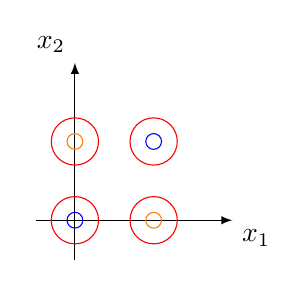
\begin{tikzpicture}[scale=1]
% Koordinatenachsen:
\draw [-latex] (-0.5,0) -- (2,0) node[below right]{$x_1$};
\draw [-latex] (0,-0.5) -- (0,2) node[above left]{$x_2$};
% Funktion:
% Punkte oben:
\draw [orange] (1,0) circle (0.1);
\draw [orange] (0,1) circle (0.1);
\draw [red] (1,0) circle (0.3);
\draw [red] (0,1) circle (0.3);
% Punkte unten
\draw [blue] (1,1) circle (0.1);
\draw [blue] (0,0) circle (0.1);
\draw [red] (1,1) circle (0.3);
\draw [red] (0,0) circle (0.3);
\end{tikzpicture}
\end{center}
Kombiniere die Ausgaben des Netzwerks aus den Ausgaben der Prototyp- bzw. Referenz-Neuronen.\\
Jedes Neuron der Hidden-Schicht bildet einen (Radius von einem) Datenpunkt dar:
\begin{center}
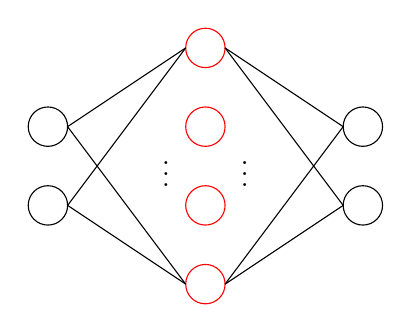
\begin{tikzpicture}[scale=.5]
\draw  (0,1) circle (0.5);
\draw  (0,-1) circle (0.5);

\draw [red] (4,3) circle (0.5);
\draw [red] (4,1) circle (0.5);
\draw [red] (4,-1) circle (0.5);
\draw [red] (4,-3) circle (0.5);

\draw  (8,1) circle (0.5);
\draw  (8,-1) circle (0.5);
\draw (0.5,1) -- (3.5,3);
\draw (0.5,1) -- (3.5,-3);
\draw (0.5,-1) -- (3.5,3);
\draw (0.5,-1) -- (3.5,-3);
\draw (4.5,3) -- (7.5,1) -- (4.5,-3);
\draw (4.5,3) -- (7.5,-1) -- (4.5,-3);
\node at (3,0) {$\vdots$};
\node at (5,0) {$\vdots$};
\end{tikzpicture}
\end{center}
Skalarprodukt:
$$z=\vec{w}^T\cdot \vec{w}$$
Distanzbasierte Aktionsgerade:
$$z=f(\vec{x},\vec{w})$$
$\to$ Vektornormen\\
$\to$ $L_2$-Norm \\
$\to$ $\boxed{z=\sqrt{(x_1-w_1)^2+\ldots + (x_n-w_n)^2}}$ (Euklidischer Abstand) … $z$ als Abstand zwischen $\vec{x}$ und $\vec{w}$.
$$y=f(z)\approx e^{-z}$$
$$\boxed{f=\exp \left( -\frac{z^2}{2 \sigma^2} \right)} \text{ Gaußfunktion}$$
\slides{NI_WS2016_Kap5_RBF}{2}

\section{Topologie}
\slides{NI_WS2016_Kap5_RBF}{3}
\section{Berechnungsvorschriften}
\slides{NI_WS2016_Kap5_RBF}{4}
\slides{NI_WS2016_Kap5_RBF}{5}
\label{berechnung_rbf}
\section{Trainingsregime}
\slides{NI_WS2016_Kap5_RBF}{6}

\subsection{Bestimmung der Gewichte von der Eingangs- zur RBF-Schicht}
\slides{NI_WS2016_Kap5_RBF}{7}
\slides{NI_WS2016_Kap5_RBF}{8}

\subsection{Bestimmung der Varianzen}
\slides{NI_WS2016_Kap5_RBF}{9}
\slides{NI_WS2016_Kap5_RBF}{10}

\subsection{Bestimmung der Gewichte von der RBF- zur Ausgabeschicht}
\slides{NI_WS2016_Kap5_RBF}{11}
$\vec{A}=f(\vec{X}, \vec{W}, \vec{\sigma})$
\slides{NI_WS2016_Kap5_RBF}{12}
Achtung bei Inverser: Elemente dürfen nicht linear abhängig sein!

\subsection{Iteratives Nachtraining}
\slides{NI_WS2016_Kap5_RBF}{13}

\subsection{Weitere mathematische Betrachtungen}
\slides{NI_WS2016_Kap5_RBF}{14}

\section{Notizen}
\lecdate{05.12.2017}
\begin{itemize}
\item Genauigkeit des Netzwerks ist geringer, je weiter die Trainingspunkte auseinander liegen (je kleiner damit die Einzugsbereiche werden).
\item Gelerntes Netzwerk bildet nur Daten in der Nähe der gelernten Punkte ab. Das kann bspw. gut sein, wenn die Frage ist, wann der Arbeitsbereich verlassen wird.
\item Bei RBF gibt es immer nur eine Hidden-Schicht!
\end{itemize}

\section{Berechnungsbeispiel}
\subsection{Gegeben}
Abbildung von 4 Merkmalen/Eingängen auf 2 Klassen.
\begin{center}
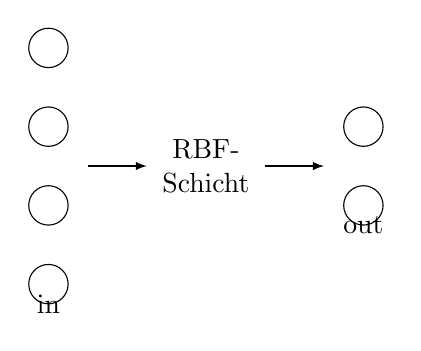
\begin{tikzpicture}[scale=.5]
\draw  (0,0) circle (0.5) node[below=.5]{in};
\draw  (0,2) circle (0.5);
\draw  (0,4) circle (0.5);
\draw  (0,6) circle (0.5);

\draw  (8,2) circle (0.5) node[below=.5]{out};
\draw  (8,4) circle (0.5);

\node at (4,3) [align=center]{RBF-\\Schicht};
\draw [-latex] (1,3) -- (2.5,3);
\draw [-latex] (5.5,3) -- (7,3);
\end{tikzpicture}
\end{center}
$$\vec{x}^1=\mtr{0\\1\\0\\1} \quad \vec{x}^2=\mtr{0\\0\\1\\0} \quad \vec{x}^3=\mtr{1\\1\\0\\0}\quad \vec{t}^1=\mtr{0\\1} \quad \vec{t}^2 =\mtr{1\\0} \quad \vec{t}^3=\mtr{0\\1}$$
\subsection{Bestimmung der RBF-Zentren}
Einfacher Ansatz: für jeden Trainingspunkt ein Zentrum.\\
Besser: Ansatz mit möglichst geringem Quantisierungsfehler.
\subsubsection{Quantisierungsfehler}
Quantisierung: Einteilung\\
$\To$ Quantisierung eines Vektorraumes durch $m$ Referenz- bzw. Codebook-Vektoren.\\
$\To$ Bestimme $\forall \vec{x} \in X$ die Differenz zwischen dem am besten passenden Referenzvektor und $\vec{x}$.\\
Referenzvektoren mit Varianz $\sigma^2 \forall$ Referenzvektoren identische Varianz angenommen:\\
Jeder Punkt hat Gaußsche Verteilung um sich. Damit ist das am besten passende (Best-Matching-Neuron) das, welches am nahsten am Punkt dran liegt. Die Differenz ist somit die Distanz (i.d.R. euklidischer Abstand) zwischen dem am besten passenden Neuron und dem betrachteten Punkt. \\
Mit $BM=(w_1,w_2)^T$ und betrachteter Punkt $\vec{x}=(x_1,x_2)^T$ ist die Differenz:
$$d(\vec{x}, BM)=\sqrt{(x_1-w_1)^2+(x_2-w_2)^2}$$
Der Einzugsbereich eines Neuron ist durch den halben Abstand zu seinen Nachbarneuronen begrenzt (Delanney-Triangulation). Den daraus erhaltenen Einzugsbereich nennt man auch Voronoi-Region.

\subsubsection{Bestimmung}
\begin{itemize}
\item Definiere einen maximalen Quantisierungsfehler $d_{max}^2=1$, der nicht überschritten werden darf.\\
$\to d^2(\vec{x}, \vec{w}^{I,RBF}) \leq 1 \;\forall x$
\item Ordne $\vec{w}_5^{I,RBF}$ Vektor $\vec{x}^1$ zu:
$$\vec{w}_5^{I,RBF}=(0,1,0,1)^T$$
\item Prüfe, ob $\vec{x}^2$ und $\vec{x}^3$ durch Referenzvektor $\vec{w}_5^{I,RBF}$ abgedeckt sind:\\
$d(\vec{x}^2,\vec{w}_5^{I,RBF}) = 3 \quad > d_{max} \;\checkmark$\\
$d(\vec{x}^3,\vec{w}_5^{I,RBF}) = 2 \quad > d_{max} \;\checkmark$
\item Ordne $\vec{w}_6^{I,RBF}$ Vektor $\vec{x}^2$ zu:
$$\vec{w}_6^{I,RBF}=(0,0,1,0)^T$$
\item Prüfe, ob $\vec{x}^3$ durch $\vec{w}_6^{I,RBF}$ abgedeckt ist:\\
$d(\vec{x}^3,\vec{w}_6^{I,RBF}) = 3 \quad > d_{max} \;\checkmark$
\item Ordne $\vec{w}_7^{I,RBF}$ Vektor $\vec{x}^3$ zu:
$$\vec{w}_7^{I,RBF}=(1,1,0,0)^T$$ 
\end{itemize}
Damit: 
\begin{center}
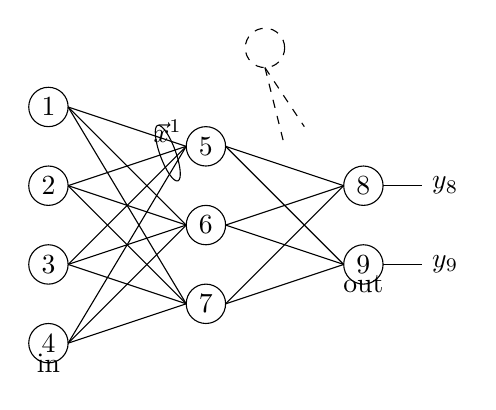
\begin{tikzpicture}[scale=.5]
\draw  (0,6) node{1} circle (0.5);
\draw  (0,4) node{2} circle (0.5);
\draw  (0,2) node{3} circle (0.5);
\draw  (0,0) node{4} circle (0.5) node[below=.5]{in};

\draw  (8,4) node{8} circle (0.5);
\draw  (8,2) node{9} circle (0.5) node[below=.5]{out};

\draw  (4,5) node{5} circle (0.5);
\draw  (4,3) node{6} circle (0.5);
\draw  (4,1) node{7} circle (0.5);

\draw (0.5,6) -- (3.5,5);
\draw (0.5,4) -- (3.5,5);
\draw (0.5,2) -- (3.5,5);
\draw (0.5,0) -- (3.5,5);

\draw (0.5,6) -- (3.5,3);
\draw (0.5,4) -- (3.5,3);
\draw (0.5,2) -- (3.5,3);
\draw (0.5,0) -- (3.5,3);

\draw (0.5,6) -- (3.5,1);
\draw (0.5,4) -- (3.5,1);
\draw (0.5,2) -- (3.5,1);
\draw (0.5,0) -- (3.5,1);
\draw [rotate=20] (4.5,3.5) ellipse (0.2 and .75) node[above=.4]{$\vec{x}^1$};

\draw (4.5,5) -- (7.5,4);
\draw (4.5,3) -- (7.5,4);
\draw (4.5,1) -- (7.5,4);

\draw (4.5,5) -- (7.5,2);
\draw (4.5,3) -- (7.5,2);
\draw (4.5,1) -- (7.5,2);

\draw (8.5,4) -- (9.5,4) node[right]{$y_8$};
\draw (8.5,2) -- (9.5,2) node[right]{$y_9$};
\draw [dashed] (5.5,7.5) circle (0.5);
\draw [dashed] (5.5,7) -- (6,5);
\draw [dashed](5.5,7) -- (6.5,5.5);
\end{tikzpicture}
\end{center}

\subsection{Ausgabevektor}
Weiterhin gegeben:
$$\vec{w}_8^{RBF,o}=\mtr{0\\1\\1} \quad \vec{w}_9^{RBF,o}=\mtr{0\\1\\0} \quad \sigma^2 = 0.5$$
Gesucht: $\vec{y}^{o}=\mtr{y_8\\y_9}$ für Eingabevektor $\vec{x}^1$\\
Rechnung: (siehe \autoref{berechnung_rbf})
\begin{itemize}
\item $z_5 = \sqrt{(x_1^1-w_{15})^2+\ldots+(x_4^1-w_{45})^2}=0$
\item $y_5=\exp\left(- \frac{z_5^2}{2 \sigma^2}\right)=1$
\item $z_6= \sqrt{(x_1^1-w_{16})^2+\ldots+(x_4^1-w_{46})^2}=\sqrt{3}$
\item $y_6 = e^{-3}$
\item $z_7 = \sqrt{(x_1^1-w_{17})^2+\ldots+(x_4^1-w_{47})^2}=\sqrt{2}$
\item $y_7 = e^{-2}$
\item $y_{RBF}=\left(1, e^{-3}, e^{-2}\right)^T$
\end{itemize}
Damit:
\begin{itemize}
\item $y_8=z_8=\vec{w}_8^T \cdot \vec{y}_{RBF} = e^{-3}+e^{-2}$
\item $y_9=z_9=\vec{w}_9^T \cdot \vec{y}_{RBF} = e^{-3}$
\end{itemize}
\subsection{Lernschritt}
Mittels Delta-Lernregel ($\eta=0,3$) einen Lernschritt für das Gewicht $w_{58}$ ausführen. Gesucht: $\Delta w_{58}$








